\chapter{Zero-Knowledge Proofs for LWE}

\section{Introduction}

LWE (Learning with error) problem is one of the fundamental lattice problems upon which lots of the lattice-based cryptography rests. LWE was first introduced by Regev in \cite{DBLP:journals/jacm/Regev09} in 2009, whose main result is a quantum reduction from lattice problems (GAPSVP and SIVP) to LWE problem. Later, researchers have found a wide range of application of it, including public-key cryptosystem \cite{DBLP:journals/jacm/LyubashevskyPR13}, universally composable oblivious transfer \cite{DBLP:conf/crypto/PeikertVW08}, etc.

LWE states that for a tuple $(A, u)$ it is hard to find a small $s$ and a small $e$ such that $u = As+e$. In this chapter, we explore a protocol in \cite{lwe} that makes use of polynomials to prove knowledge of $s$ and $e$ with small elements that satisfy:
$$
    As + e = u
$$

\begin{definition}[Relation $R_{LWE}$]
The relation $R_{LWE}$ is the sets of tuples
$$
    (\mathbb{X}, \mathbb{W}) = ((\mathbb{F}, n, m, A, u), (s, e))
$$ 
such that $A \in \mathbb{F}^{n \times m}$, $u \in \mathbb{F}^{n}$, $s \in \{-1, 0, 1\}^{m}$, $e \in \{-1, 0, 1\}^{n}$ and $As + e = u$.
\end{definition}


\section{LWE Protocol}


Prover $\mathcal{P}$'s input: $A \in \mathbb{F}^{n \times m}$, $u \in \mathbb{F}^{n}$, $s \in \{-1, 0, 1\}^{m}$ and $e \in \{-1, 0, 1\}^{n}$ such that $u = As + e$.

Verifier $\mathcal{V}$'s input: $A \in \mathbb{F}^{n \times m}$, $u \in \mathbb{F}^{n}$.

The protocol proceeds as follows.



\begin{itemize}
    \item $\mathcal{P}$ samples $t \leftarrow \mathbb{F}^{m}$ and computes the polynomials:
\begin{equation}
\label{eq:lwe3}
    f(X) = tX+s = f_1 X + f_0
\end{equation}
\begin{equation}
\label{eq:lwe4}
    d(X)=u-Af(X) = d_1 X + d_0
\end{equation}
If the prover is honest, $(f_1, f_0) \in (\mathbb{F}^m, \mathbb{F}^m)$ should equal to $(t, s)$ and $(d_1, d_0) \in (\mathbb{F}^n, \mathbb{F}^n)$ should equal to $(-At, u-As)$.

    \item $\mathcal{P}$ computes the polynomials:
\begin{equation}
\label{eq:lwe1}
    \frac{1}{X} f(X) \circ [f(X) - 1^m] \circ [f(X) + 1^m] = v_2X^2 + v_1X + v_0
\end{equation}
\begin{equation}
\label{eq:lwe2}
    \frac{1}{X} d(X) \circ [d(X) - 1^n] \circ [d(X) + 1^n] = w_2X^2 + w_1X + w_0
\end{equation}
where $(v_2, v_1, v_0) \in (\mathbb{F}^m, \mathbb{F}^m, \mathbb{F}^m)$ and $(w_2, w_1, w_0) \in (\mathbb{F}^n, \mathbb{F}^n, \mathbb{F}^n)$.

    \item $\mathcal{P}$ samples $r_2, r_1, r_0 \leftarrow \mathbb{F}^N$.


    \item $\mathcal{P}$ computes the encodings:
\begin{equation*}
    H_2^\prime = \widetilde{\textsc{Enc}}(H_2, r_2) \in \mathbb{F}^{2N}
\end{equation*}
\begin{equation*}
    H_1^\prime = \widetilde{\textsc{Enc}}(H_1, r_1) \in \mathbb{F}^{2N}
\end{equation*}
\begin{equation*}
    H_0^\prime = \widetilde{\textsc{Enc}}(H_0, r_0) \in \mathbb{F}^{2N}
\end{equation*}
where, 
\begin{align*}
    \widetilde{\textsc{Enc}}(H, r) &= (\textsc{Enc}(H) + r, r) \\ 
    H_2 &= f_2, v_2, w_2
    \in \mathbb{F}^{2m+n} \quad (f_2 = 0^m) \\
    H_1 &= f_1, v_1, w_1
    \in \mathbb{F}^{2m+n} \\
    H_0 &= f_0, v_0, w_0
    \in \mathbb{F}^{2m+n}
\end{align*}

    \item $\mathcal{P}$ sends $H_2^\prime, H_1^\prime, H_0^\prime$ to $\mathcal{V}$, and $\mathcal{V}$ has point query access to each of these messages.
    
    \item $\mathcal{V}$ samples a random challenge $x \leftarrow \mathbb{F}^*$ and sends it to $\mathcal{P}$.
    
    \item $\mathcal{P}$ computes $\overline{H} = x^2H_2 + xH_1 + H_0 \in \mathbb{F}^{2m+n}$.
    
    \item $\mathcal{P}$ computes $\overline{r} = x^2r_2 + xr_1 + r_0 \in \mathbb{F}^{2m+n}$.

    \item $\mathcal{P}$ sends $\overline{H}$ and $\overline{r}$ to $\mathcal{V}$.

    \item $\mathcal{V}$ samples an indices set $I$ with $\lambda$ indices from space $[2N]$ with the restriction that $\forall i_1, i_2 \in I, |i_1 - i_2| \neq N$. Then for each index $i$, $\mathcal{V}$ will check whether the following equation holds through point queries to $H_2^\prime, H_1^\prime$ and $H_0^\prime$.
\begin{equation}
\label{eq:lwe5}
    \widetilde{\textsc{Enc}}(\overline{H}, \overline{r})[i] 
    \stackrel{?}{=} 
    H_2^\prime[i] x^2 + H_1^\prime[i] x + H_0^\prime[i]
\end{equation}

    \item Let $(\overline{f}, \overline{g}, \overline{h}) \leftarrow \overline{H}$, where $(\overline{f}, \overline{g}, \overline{h}) \in (\mathbb{F}^m, \mathbb{F}^m, \mathbb{F}^n)$. 
    
    \item $\mathcal{V}$ computes $\overline{d} = u - A\overline{f}$.

    \item $\mathcal{V}$ will check whether the following equation holds:
\begin{equation}
\label{eq:lwe6}
    \overline{g} \overset{?}{=} \frac{1}{x} (\overline{f} \circ [\overline{f} - 1^m] \circ [\overline{f} + 1^m])
\end{equation}
\begin{equation}
\label{eq:lwe7}
    \overline{h} \overset{?}{=} \frac{1}{x} (\overline{d} \circ [\overline{d} - 1^n] \circ [\overline{d} + 1^n])
\end{equation}
    

\end{itemize}

\begin{lemma}
\label{lemma:lwepc}

LWE = ($\mathcal{P}$, $\mathcal{V}$) has \textbf{perfect completeness}.

\end{lemma}
\begin{proof}

Equation \ref{eq:lwe5} is checking whether $\overline{H}$ and $\overline{r}$ is a correct linear combination of $H_2^\prime, H_1^\prime$ and $H_0^\prime$. If the prover $\mathcal{P}$ is honest, it will succeed.


For equation \ref{eq:lwe6}, because $\mathcal{P}$ computes it honestly according to equation \ref{eq:lwe1}, it will succeed.
\begin{align*}
    \overline{g} 
    &= v_2x^2 + v_1x + v_0 \\
    &= \frac{1}{x} f(x) \circ [f(x) - 1^m] \circ [f(x) + 1^m] \\
    &= \frac{1}{x} (\overline{f} \circ [\overline{f} - 1^m] \circ [\overline{f} + 1^m]) 
\end{align*}

For equation \ref{eq:lwe7}, because $\mathcal{P}$ computes it honestly according to equation \ref{eq:lwe2}, it will succeed.
\begin{align*}
    \overline{h} 
    &= w_2x^2 + w_1x + w_0 \\
    &= \frac{1}{x} d(x) \circ [d(x) - 1^m] \circ [d(x) + 1^m] \\
    &= \frac{1}{x} (\overline{d} \circ [\overline{d} - 1^m] \circ [\overline{d} + 1^m]) 
\end{align*}

\end{proof}

We cite the following lemma from paper \cite{lwe} to complete the soundness proof.

\begin{lemma}
\label{lemma:lweseproof}

If there exist some $c^* \in \mathbb{F}^3$ such that $d(C, c^*E^*) \ge \frac{\delta}{10}$, then
$$
    Pr\biggl[ d(C, (x^2, x, 1)E^*) \le \frac{\delta}{30} \biggr] \le \frac{2}{q-1}
$$
where $q$ is the size of the underlying field, $d$ is the relative distance function and $C$ is the codeword.

\end{lemma}

\begin{lemma}
\label{lemma:lwese}

LWE = ($\mathcal{P}$, $\mathcal{V}$) has has soundness error at most 
$$
    \max
    \biggl\{
    \frac{2}{q} + \frac{q-2}{q}(1 - \delta)^\lambda, 
    \frac{2}{q-1} + \frac{q-3}{q-1}(1 - \frac{29\delta}{30})^\lambda,
    (1 - \frac{7\delta}{10})^\lambda
    \biggr\}
$$
where $q$ is the size of the underlying field and $\delta$ is the relative distance of the codeword represented by the encoding function $\widetilde{\textsc{Enc}}$.

\end{lemma}
\begin{proof}

Suppose $H_2^\prime$, $H_1^\prime$ or $H_0^\prime$ is at least $\frac{\delta}{10}$ far away from a valid codeword. Without loss of generality, we assume $H_2^\prime$ is not a valid codeword. Then let $c^* = (1, 0, 0)$, according to lemma \ref{lemma:lweseproof}, the probability that a structured linear combination of $H_2^\prime$, $H_1^\prime$ and $H_0^\prime$ is $\frac{\delta}{30}$ close to a codeword is bound by $\frac{2}{q-1}$. Then the probability that they are not $\frac{\delta}{30}$ close to a codeword is $\frac{q-3}{q-1}$. In this case, the probability that verification equation \ref{eq:lwe5} passed is $(1 - \frac{29\delta}{30})^\lambda$. Therefore, the soundness error is at most $\frac{2}{q-1} + \frac{q-3}{q-1}(1 - \frac{29\delta}{30})^\lambda$.

Otherwise, $H_2^\prime$, $H_1^\prime$ and $H_0^\prime$ are $\frac{\delta}{10}$ close to a valid codeword, and it is possible to decode them to a instance/witness $(\mathbb{X}, \mathbb{W}) = ((\mathbb{F}, n, m, A, u), (s, e))$. 

Suppose the malicious prover $\mathcal{P}$ does not follow the protocol honestly and sends incorrect messages. 
\begin{itemize}

    \item If one of the following condition satisfied ($\overline{f}, \overline{g}$, or $\overline{h}$ is incorrect),
    $$\overline{f} = x^2f_2 + xf_1 + f_0$$
    $$\overline{g} = x^2g_2 + xg_1 + g_0$$
    $$\overline{h} = x^2h_2 + xh_1 + h_0$$
    then according to the relative distance property of the encoding function $\widetilde{\textsc{Enc}}$, 
    at least $\delta$ portion of $\widetilde{\textsc{Enc}}(\overline{H}, \overline{r})$ and
    $x^2\widetilde{\textsc{Enc}}(H_2, r_2) + x\widetilde{\textsc{Enc}}(H_1, r_1) + \widetilde{\textsc{Enc}}(H_0, r_0)$.
    And since $\widetilde{\textsc{Enc}}(H_i, r_i)$ and $H_i^\prime$ are $\frac{\delta}{10}$ close to each other, at least $\frac{7\delta}{10}$ portion of $\widetilde{\textsc{Enc}}$ and 
    $H_2^\prime x^2 + H_1^\prime x + H_0^\prime$ will be different. The probability that all $\lambda$ random checks (equation \ref{eq:lwe5}) are passed is at most $(1 - \frac{7\delta}{10})^\lambda$.
    
    \item If $f_2, f_1, f_0, v_2, v_1, v_0, w_2, w_1$ or $w_0$ is incorrect (different from equation \ref{eq:lwe1}, \ref{eq:lwe2}, \ref{eq:lwe3}, \ref{eq:lwe4}), denote the incorrect polynomial as $f^\prime$, $g^\prime$ or $h^\prime$. Since $f$ and $f^\prime$, $g$ and $g^\prime$ or $h$ and $h^\prime$ are polynomials with degree at most 2. According to the Schwartz-Zippel lemma, they can agree on at most 2 evaluation points. And since evaluation point $x$ is sampled randomly, the probability this event happens is at most $\frac{2}{q}$. If this event does not happen, then according to the relative distance property of the encoding function $\widetilde{\textsc{Enc}}$, at least $\delta$ portion of $\widetilde{\textsc{Enc}}(\overline{H}, \overline{r})$ and $H_2^\prime x^2 + H_1^\prime x + H_0^\prime$ will be different. The probability that all $\lambda$ random checks (equation \ref{eq:lwe5}) are passed is at most $(1 - \delta)^\lambda$. Therefore, the soundness error is at most $\frac{2}{q} + \frac{q-2}{q}(1 - \delta)^\lambda$.


\end{itemize}

Otherwise, the prover $\mathcal{P}$ follows the protocol honestly. Suppose $(\mathbb{X}, \mathbb{W}) = ((\mathbb{F}, n, m, A, u), (s, e))$ is not in relation $R_{LWE}$. Then at least one of the following conditions is satisfied:
\begin{itemize}
    \item $s \notin \{-1, 0, 1\}^{m}$: Then there is an $v_{-1} X^{-1}$ term in $\frac{1}{X} f(X) \circ [f(X) - 1^m] \circ [f(X) + 1^m]$. Therefore, polynomial $g$ is incorrect, denoting the incorrect polynomial as $g^\prime$. $g$ and $g^\prime$ are polynomials with degree 2. According to the Schwartz-Zippel lemma, they can agree on at most 2 evaluation points. And since evaluation point $x$ is sampled randomly, the probability this event happens so that equation \ref{eq:lwe6} is satisfied is at most $\frac{2}{q}$. 
    
    \item $e \notin \{-1, 0, 1\}^{n}$: Then there is an $w_{-1} X^{-1}$ in $\frac{1}{X} d(X) \circ [d(X) - 1^n] \circ [d(X) + 1^n]$. Therefore, polynomial $h$ is incorrect, denote the incorrect polynomial as $h^\prime$. $h$ and $h^\prime$ are polynomials with degree 2. According to the Schwartz-Zippel lemma, they can agree on at most 2 evaluation points. And since evaluation point $x$ is sampled randomly, the probability this event happens so that equation \ref{eq:lwe7} is satisfied is at most $\frac{2}{q}$. 
    
    \item $u \neq As + e$: Then polynomial $d$ will be incorrect, denote the incorrect polynomial as $d^\prime$. Then, $\overline{h}$ and $\frac{1}{x} (d^\prime \circ [d^\prime - 1^n] \circ [d^\prime + 1^n])$ can agree on at most 2 evaluation points. And since evaluation point $x$ is sampled randomly, the probability this event happens so that equation \ref{eq:lwe7} is satisfied is at most $\frac{2}{q}$. 
    
\end{itemize}


\end{proof}

\begin{lemma}
\label{lemma:lwezk}

LWE = ($\mathcal{P}$, $\mathcal{V}$) is semi-honest verifier zero-knowledge.

\end{lemma}
\begin{proof}

The  verifier $\mathcal{V}$'s view includes $(x, \overline{f}, \overline{g}, \overline{h}, \overline{r})$ and $(H_2^\prime[i], H_1^\prime[i], H_0^\prime[i])$ for $\forall i \in I$. The simulator $\mathcal{S}(A, u)$ can generate the verifier $\mathcal{V}$'s view as follows:

\begin{itemize}

    \item $\mathcal{S}$ samples $x \in \mathbb{F}$ uniformly at random.

    \item $\mathcal{S}$ samples $\overline{f} \in \mathbb{F}^m$ uniformly at random.
    
    \item $\mathcal{S}$ computes $\overline{d} = u - A\overline{f} \in \mathbb{F}^n$.
    
    \item $\mathcal{S}$ computes $\overline{g} = \frac{1}{x} (\overline{f} \circ [\overline{f} - 1^m] \circ [\overline{f} + 1^m]) \in \mathbb{F}^m$.
    
    \item $\mathcal{S}$ computes $\overline{h} = \frac{1}{x} (\overline{d} \circ [\overline{d} - 1^n] \circ [\overline{d} + 1^n]) \in \mathbb{F}^n$.
    
    \item $\mathcal{S}$ samples $r_2, r_1, r_0 \in \mathbb{F}^N$ uniformly at random.
    
    \item $\mathcal{S}$ computes $\overline{r} = x^2 r_2 + x r_1 + r_0 \in \mathbb{F}^N$.

    \item $\mathcal{S}$ samples $f_2, f_1 \in \mathbb{F}^m$ uniformly at random.

    \item $\mathcal{S}$ samples $v_2, v_1 \in \mathbb{F}^m$ uniformly at random.
    
    \item $\mathcal{S}$ samples $w_2, w_1 \in \mathbb{F}^n$ uniformly at random.
    
    \item $\mathcal{S}$ computes $f_0 = \overline{f} - x^2 f_2 - x f_1 \in \mathbb{F}^m$.
    
    \item $\mathcal{S}$ computes $v_0 = \overline{g} - x^2 v_2 - x v_1 \in \mathbb{F}^m$.

    \item $\mathcal{S}$ computes $w_0 = \overline{h} - x^2 w_2 - x w_1 \in \mathbb{F}^n$.  
    
    \item $\mathcal{S}$ computes $H_2^\prime = \widetilde{\textsc{Enc}}(H_2, r_2) \in \mathbb{F}^{2N}$, where $H_2 = f_2, v_2, w_2$.

    \item $\mathcal{S}$ computes $H_1^\prime = \widetilde{\textsc{Enc}}(H_1, r_1) \in \mathbb{F}^{2N}$, where $H_1 = f_1, v_1, w_1$.

    \item $\mathcal{S}$ computes $H_0^\prime = \widetilde{\textsc{Enc}}(H_0, r_0) \in \mathbb{F}^{2N}$, where $H_0 = f_0, v_0, w_0$.
    
    \item $\mathcal{S}$ outputs $(x, \overline{f}, \overline{g}, \overline{h}, \overline{r})$ and $(H_2^\prime[i], H_1^\prime[i], H_0^\prime[i])$ for $\forall i \in I$.
\end{itemize}

Variable $x$ is simulated for any fixed choice of randomness and is indistinguishable from the real transcripts.

For the simulated transcripts, $\overline{f}$ is randomly sampled. For the real transcripts, $\overline{f}$ also looks random because $\overline{f} = tx + s$ where $t$ is randomly sampled.

For both the simulated transcripts and the real transcripts, $\overline{g}$ equals to $\frac{1}{x} (\overline{f} \circ [\overline{f} - 1^m] \circ [\overline{f} + 1^m])$. Since $\overline{f}$ looks random, they are indistinguishable from each other.

For both the simulated transcripts and the real transcripts, $\overline{h}$ equals to $\frac{1}{x} (\overline{d} \circ [\overline{d} - 1^n] \circ [\overline{d} + 1^n])$. Since $\overline{d} = u - A\overline{f}$ looks random, they are indistinguishable from each other.

For both the simulated transcripts and the real transcripts, $r_2, r_1, r_0$ are randomly sampled. Therefore, $\overline{r} = x^2 r_2 + x r_1 + r_0$ looks random.

In the real transcripts, individual elements in $H_2^\prime, H_1^\prime$, and $H_0^\prime$ look random because the mask $r_2, r_1, r_0$ are randomly sampled and all other elements are hidden by the random mask. In the simulated transcripts, for the same reason, $H_2^\prime, H_1^\prime$, and $H_0^\prime$ also look random. Therefore, as long as $\forall i_1, i_2 \in I, |i_1 - i_2| \neq N$, they are indistinguishable from each other.
\qedsymbol{}
\end{proof}


\section{Benchmark}

In practice, we use Merkle tree commitment to compile the IOP to a real argument system as well. We implement the above mentioned protocol in Rust. We benchmark the above LWE protocol on a computer with
Intel \textregistered \, Core  \textsuperscript{TM} i7-7700HQ CPU @ 2.80GHz (Kabylake), L1 cache: 128KB, L2 cache: 256KB and L3 cache: 6MB. There are 8 physical CPU cores available on this machine. The runtimes are summarized in the table \ref{table:benchmark-lwe}.


As $n$ and $m$ increase, it generally requires more time to complete
the committing phase for the prover and the checking phase for the verifier. Also, larger $n$ and $m$ will result in a larger proof size.




\begin{table}[h!]
\centering
\begin{tabular}{|c|m{4em}|m{4em}|m{4em}|m{4em}|m{5em}|}
\hline

\multicolumn{1}{|l|}{n}                     & m   & Code Length  & Prover Time {[}ms{]} & Verifier Time {[}ms{]} & Proof Size {[}bytes{]} \\ \hline\hline
\multirow{5}{*}{128}                        & 128 & 661 & 41                   & 36                     & 10624                                         \\ \cline{2-6} 
                                            & 256 & 1101 & 70                  & 54                     & 12448                                         \\ \cline{2-6} 
                                            & 512 & 1982 & 111                  & 79                    & 14496                                         \\ \cline{2-6} 
                                            & 1024 & 3743 & 214                  & 127                    & 19392                                         \\ \cline{2-6} 
                                            & 2048 & 7266 & 426                  & 261                    & 28384                                         \\ \hline
\multirow{5}{*}{256}                        & 128  & 881 & 57                   & 49                     & 10624                                         \\ \cline{2-6} 
                                            & 256  & 1321 & 92                  & 74                    & 12448                                         \\ \cline{2-6} 
                                            & 512  & 2202 & 193                  & 114                    & 15296                                         \\ \cline{2-6} 
                                            & 1024 & 3963 & 272                  & 196                    & 19392                                         \\ \cline{2-6} 
                                            & 2048 & 7486 & 539                  & 382                    & 28384                                         \\ \hline
\multirow{5}{*}{512}                        & 128  & 1321 & 152                  & 94                    & 11424                                         \\ \cline{2-6} 
                                            & 256  & 1762 & 149                  & 124                    & 12448                                         \\ \cline{2-6} 
                                            & 512  & 2642 & 254                  & 209                    & 15296                                         \\ \cline{2-6} 
                                            & 1024 & 4404 & 465                  & 337                    & 20192                                         \\ \cline{2-6} 
                                            & 2048 & 7926 & 732                 & 590                   & 28384                                         \\ \hline
\multicolumn{1}{|l|}{\multirow{5}{*}{1024}} & 128  & 2202 & 152                  & 114                    & 12224                                         \\ \cline{2-6} 
\multicolumn{1}{|l|}{}                      & 256  & 2642 & 221                  & 197                    & 13248                                         \\ \cline{2-6} 
\multicolumn{1}{|l|}{}                      & 512  & 3523 & 440                  & 309                    & 15296                                         \\ \cline{2-6} 
\multicolumn{1}{|l|}{}                      & 1024 & 5284 & 685                 & 553                   & 20192                                         \\ \cline{2-6} 
\multicolumn{1}{|l|}{}                      & 2048 & 8807 & 1297                 & 1140                   & 29184                                         \\ \hline
\multicolumn{1}{|l|}{\multirow{5}{*}{2048}} & 128  & 3963 & 279                  & 198                    & 12224                                         \\ \cline{2-6} 
\multicolumn{1}{|l|}{}                      & 256  & 4404 & 464                  & 342                    & 14048                                         \\ \cline{2-6} 
\multicolumn{1}{|l|}{}                      & 512  & 5284 & 761                 & 595                    & 16096                                         \\ \cline{2-6} 
\multicolumn{1}{|l|}{}                      & 1024 & 7046 & 1199                 & 1109                   & 20192                                         \\ \cline{2-6} 
\multicolumn{1}{|l|}{}                      & 2048 & 10568 & 2463                 & 2096                   & 29184                                         \\ \hline
\end{tabular}
\caption{Runtime of LWE protocol with 1 thread and 200 test tuples. The soundness error is around 0.007.}
\label{table:benchmark-lwe}
\end{table}



\begin{figure}[h]
    \centering
    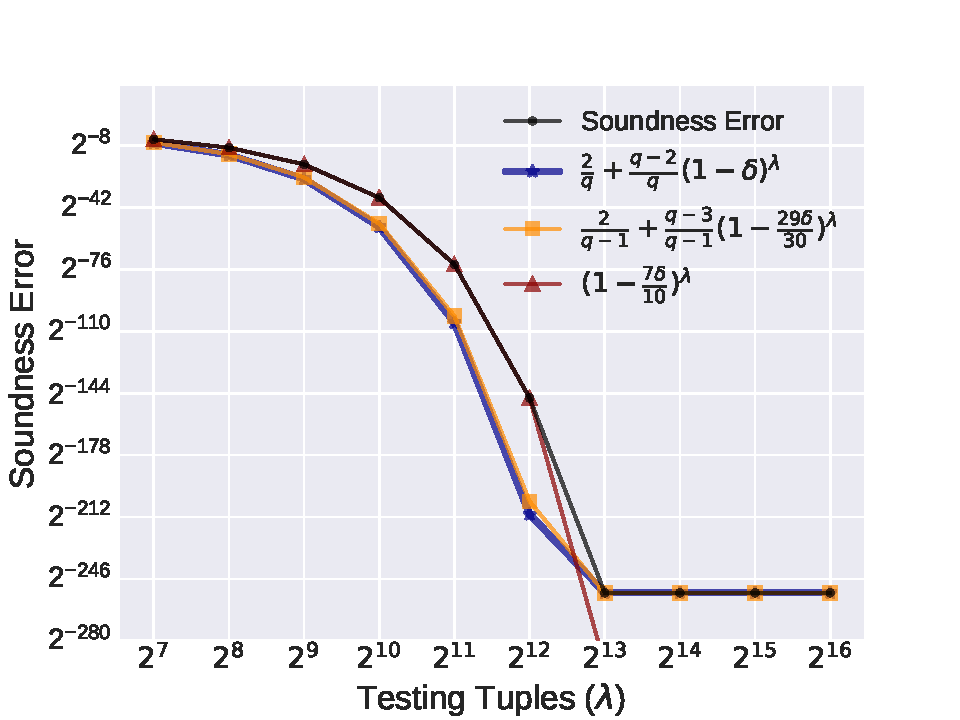
\includegraphics[width=1\textwidth]{graph/se.pdf}
    \caption{Soundness Error of LWE Protocol}
    \label{fig:se}
\end{figure}

Also figure \ref{fig:se} shows the relation between soundness error and the number of testing tuples ($\lambda$). As mentioned in lemma \ref{lemma:lwese}, the soundness error is the maximum value of three individual terms. Figure \ref{fig:se} labels these terms using lines with different colors. When $\lambda$ is small, the soundness error is dominated by $(1 - \frac{7\delta}{10})^\lambda$.
As $\lambda$ increasing, the soundness is decreasing and is gradually dominated by $\frac{2}{q-1}$. Hence, the minimum possible soundness is actually independent of the number of testing tuples ($\lambda$), and is determined solely by the field size. In our benchmark, we use a field with a size roughly equal to $2^{32}$, therefore, the minimum possible soundness error is around $2^{-32}$.
